\section{User Manual of ab4.py}
The Python command line interface application ab4.py computes the solution of both sides of \(\frac{1}{x} - \frac{1}{x + 1} = \frac{1}{x (x + 1)}\) depending on the value for x and the desired mantissa length of the floating point arithmetic. \\
After starting, ab4.py first prints out the machine precision for np.float16, np.float32 and np.float64 (see figure \ref{fig:cmd_epsilon}).
\begin{figure}[h]
    \centering
        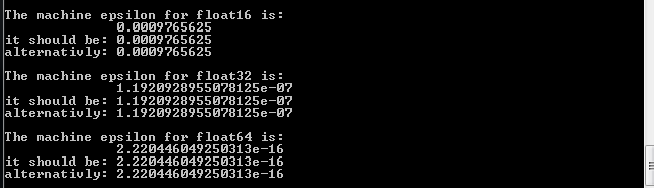
\includegraphics[width=0.9\textwidth]{graphics/cmd_epsilon}
    \caption{command line output of ab4.py regarding different floating types}\label{fig:cmd_epsilon}
\end{figure}\\
Then, the user may input the values for x and the mantissa length. ab4.py will print the solution of both sides of the equation and the absolute and the relative error. Two corresponding plot for both errors with varied mantissa length (from 1 to 28) are also drawn. See figure \ref{fig:cmd_example} for an example input and output.
\begin{figure}[h]
    \centering
        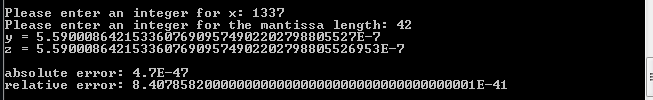
\includegraphics[width=0.9\textwidth]{graphics/cmd_example}
    \caption{example input with x = 1337 and mantissa length = 42 and its output}\label{fig:cmd_example}
\end{figure}\\
The user may exit the application by typing "exit" or leaving the line empty when asked to enter the value for x.